\documentclass[aspectratio=169]{beamer}
\usepackage{will_handley_beamer}
\usepackage{title_page}

\title{The scaling frontier of nested sampling}
\date{1\textsuperscript{st} July 2024}

\begin{document}

\begin{frame}
    \titlepage
\end{frame}

\begin{frame}
    \frametitle{Recap: the nested sampling meta-algorithm}
    \begin{columns}
        \column{0.5\textwidth}
        \begin{itemize}
            \item Start with $n_\text{live}$ random prior samples $\theta\sim\C[1]{\pi}$.
            \item Delete lowest likelihood sample, and replace with a new one at higher value.
            \item The ``live points'' steadily contract around the peak(s) of the function.
            \item We can use this evolution to estimate volume \emph{probabilistically}.
            \item At each iteration, the contours contract by $\sim\frac{1}{n_\text{live}}\only<5->{\pm \frac{1}{n_\text{live}}}$ of their volume.
            \item This is an exponential contraction, so
                \[  \C[3]{\mathcal{Z}} = \int \C[2]{\mathcal{L}} \C[1]{\pi} d\theta \approx \sum_{\mathclap{i\in\text{dead}}} \C[2]{\mathcal{L}}_i \Delta X_i, \quad X_i = e^{-\only<5->{(}i\only<5->{\pm\sqrt{i})}/n_\text{live}} \]
        \end{itemize}
        \column{0.5\textwidth}
        \includegraphics<1|handout:0>[width=\textwidth,page=1]{figures/himmelblau}%
        \includegraphics<2|handout:0>[width=\textwidth,page=2]{figures/himmelblau}%
        \includegraphics<3|handout:0>[width=\textwidth,page=3]{figures/himmelblau}%
        \includegraphics<4-         >[width=\textwidth,page=4]{figures/himmelblau}%
    \end{columns}
\end{frame}

\begin{frame}
    \frametitle{Kullback Leibler divergence (or entropy $H$ or, information gain)}
    \begin{columns}
        \column{0.5\textwidth}
        \begin{itemize}
            \item The KL divergence between \C[1]{prior $\pi$} and \C[0]{posterior $\mathcal{P}$} is is defined as:
                \[\mathcal{D}_\text{KL} = \av[{\C[0]{\mathcal{P}}}]{\log\frac{\C[0]{\mathcal{P}}}{\C[1]{\pi}}} = \int \C[0]{\mathcal{P}}(\theta) \log \frac{\C[0]{\mathcal{P}}(\theta)}{\C[1]{\pi}(\theta)}d\theta.\]
            \item Whilst not a distance, $\mathcal{D}=0$ when $\C[0]{\mathcal{P}}=\C[1]{\pi}$.
            \item Occurs in the context of machine learning as an objective function for training functions.
            \item In Bayesian inference it can be understood as a log-ratio of ``volumes'':
                \[ \mathcal{D}_\text{KL} \approx \log \frac{V_{\C[1]{\pi}}}{V_{\C[0]{\mathcal{P}}}}.\]
                (this is exact for top-hat distributions).
        \end{itemize}
        \column{0.5\textwidth}
        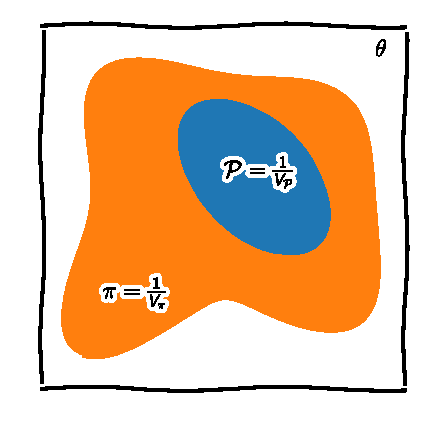
\includegraphics{figures/volumes.pdf}
    \end{columns}
\end{frame}

\begin{frame}
    \frametitle{How fast in nested sampling?}
    \student{zixiao_hu}{Zixiao Hu}{MSci 2023}
    \begin{columns}
        \column{0.75\textwidth}
        \[
            \boxed{
                T = T_{\C[2]{\mathcal{L}}} \times \underbrace{
                    \overbrace{
                        n_\text{live}  \times \mathcal{D}_\text{KL}
                    }^{\displaystyle n_\text{dead}}
                    \times f_\text{sampler}
                }_{\displaystyle n_{\C[2]{\mathcal{L}}}},
            }
        \]
        \vspace{-10pt}
        \begin{itemize}
            \item NS compresses the volume $X$ of the live points from prior $X=1$ to posterior $X = e^{-\mathcal{D}_\text{KL}}$.
            \item It does this exponentially so at iteration $i$, $X_i = e^{-i/n_\text{live}}$
            \item Need $e^{-n_\text{dead}/n_\text{live}}\sim e^{-\mathcal{D}_\text{KL}}\Rightarrow \boxed{n_\text{dead}\sim n_\text{live}\times\mathcal{D}_\text{KL}}$.
            \item It takes a $f_\text{sampler}$ likelihood evaluations to generate a new live point, so $n_{\C[2]{\mathcal{L}}} = n_\text{dead}\times f_\text{sampler}$
            \item It takes $T_{\C[2]{\mathcal{L}}}$ seconds to call the likelihood, so $T=T_{\C[2]{\mathcal{L}}}\times n_{\C[2]{\mathcal{L}}}$
        \end{itemize}
        \begin{exampleblock}{Further reading~\arxiv{2312.00294}}
            \texttt{aeons}: approximating the end of nested sampling, (Zixiao Hu et al) 
        \end{exampleblock}
        \column{0.25\textwidth}
        \vspace{8pt}
        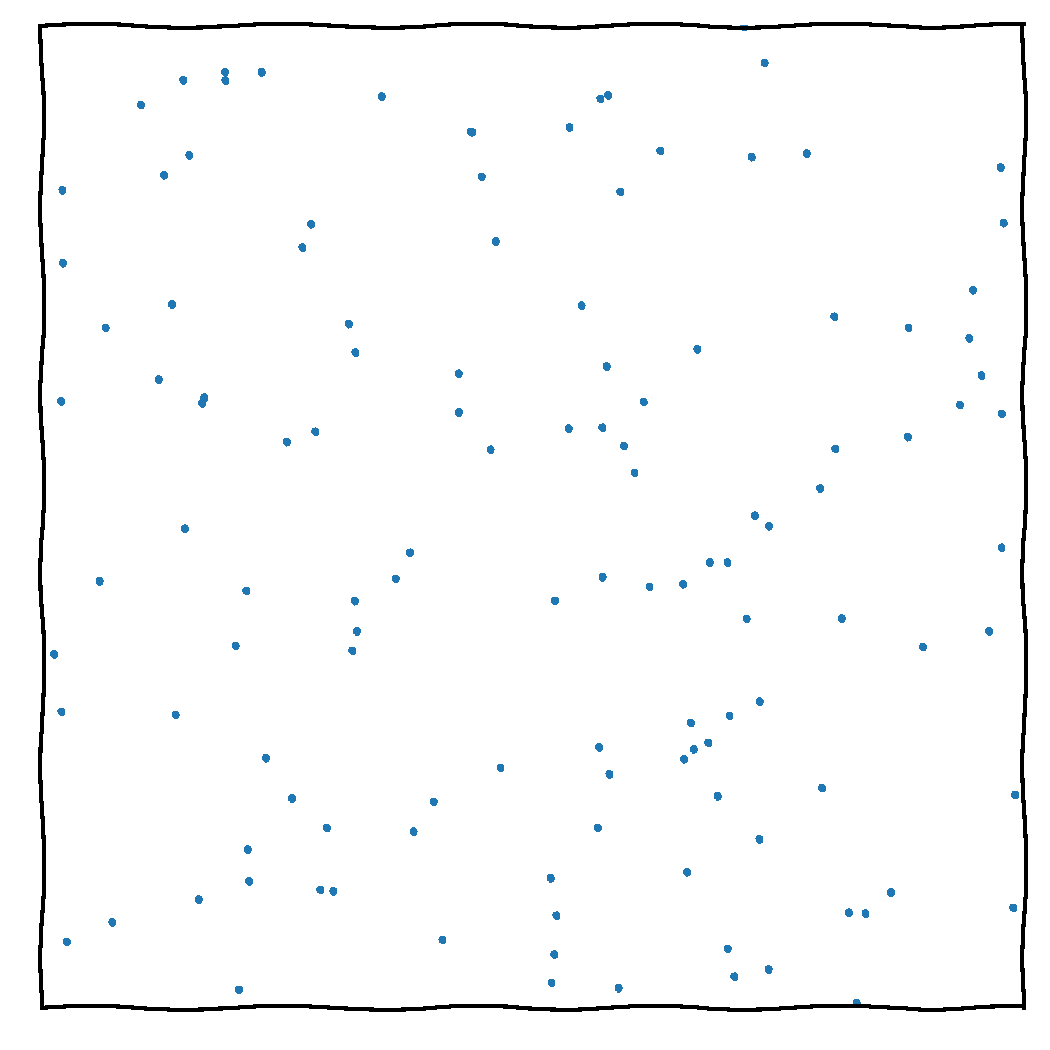
\includegraphics[width=\textwidth,page=1]{figures/himmelblau}
        \includegraphics[width=\textwidth,page=6]{figures/himmelblau}
    \end{columns}
\end{frame}

\begin{frame}
    \frametitle{How accurate is nested sampling?}
    \student{lukas_hergt}{Lukas Hergt}{PhD 2020}
    \begin{columns}
        \column{0.75\textwidth}
        \[ \boxed{\sigma(\log\C[3]{\mathcal{Z}}) \approx \sqrt{\mathcal{D}_\text{KL}/n_\text{live}}} \]
        \begin{itemize}
            \item From the Occam's razor equation~\arxiv{2102.11511}:
                \[\log \C[3]{\mathcal{Z}} = \av[{\C[0]{\mathcal{P}}}]{\log\C[2]{\mathcal{L}}} - \mathcal{D}_\text{KL}\]
            \item The dominant error is in the estimation of compression $\mathcal{D}_\text{KL}$
            \item At each iteration, compress by $\exp(-\frac{1}{n_\text{live}} \pm \frac{1}{n_\text{live}})$
            \item After $n_\text{dead}$ iterations, compressed by $e^{-\frac{n_\text{dead}}{n_\text{live}} \pm \frac{\sqrt{n_\text{dead}}}{n_\text{live}}} = e^{-\mathcal{D}_\text{KL}}$
            \item As before $n_\text{dead}\sim n_\text{live}\times\mathcal{D}_\text{KL}$
            \item $\sigma(\log\C[3]{\mathcal{Z}}) = \sigma (\mathcal{D}_\text{KL}) = \frac{\sqrt{n_\text{dead}}}{n_\text{live}}= \sqrt{\frac{\mathcal{D}_\text{KL}}{n_\text{live}}}$
        \end{itemize}
        \column{0.25\textwidth}
        \vspace{8pt}
        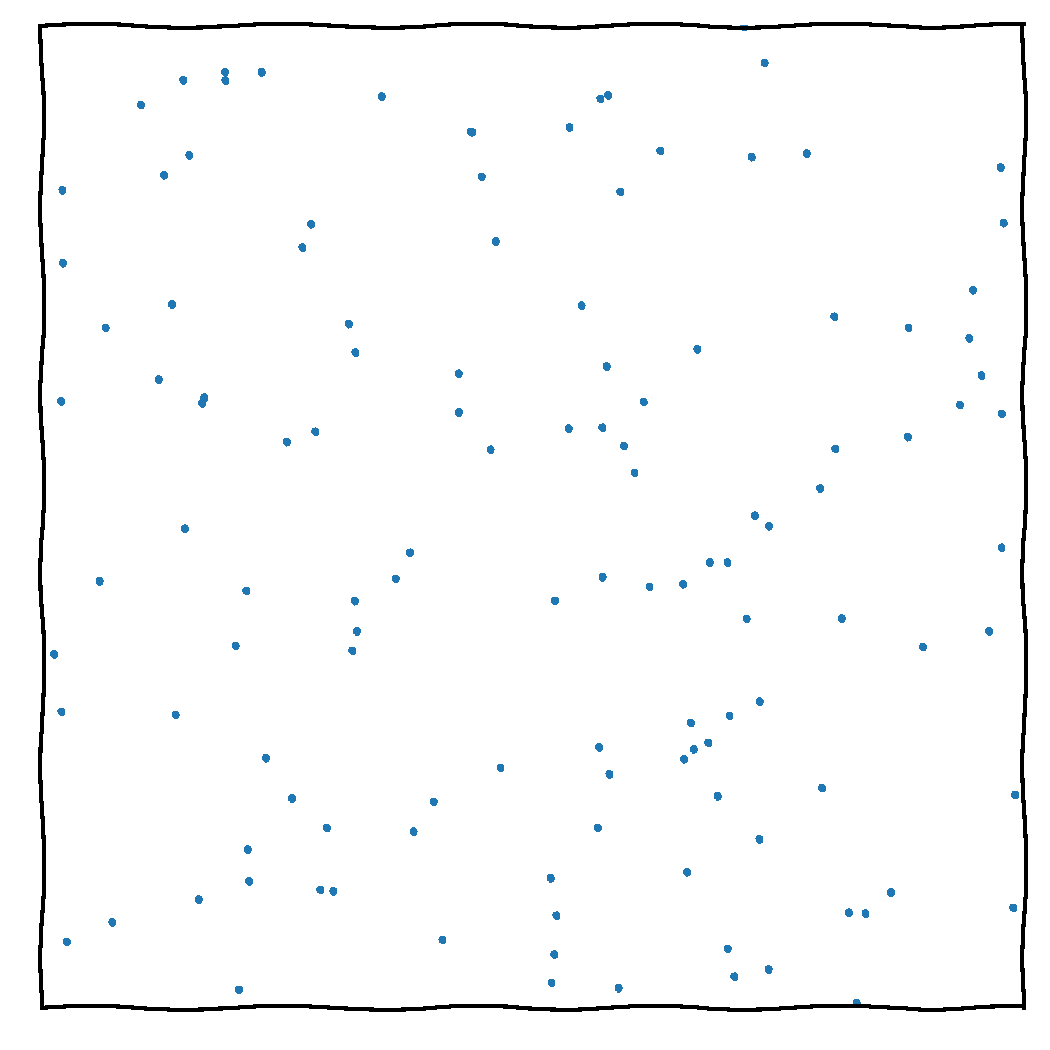
\includegraphics[width=\textwidth,page=1]{figures/himmelblau}
        \includegraphics[width=\textwidth,page=6]{figures/himmelblau}
    \end{columns}
\end{frame}

\begin{frame}
    \frametitle{The scaling frontier of nested sampling}
    \begin{columns}[t]
        \column{0.47\textwidth}
        \begin{block}{How fast in nested sampling?}
            \[ \boxed{T = T_{\C[2]{\mathcal{L}}} \times n_\text{live} \times \mathcal{D}_\text{KL} \times f_\text{sampler}} \]
        \end{block}
        \column{0.43\textwidth}
        \begin{block}{How accurate is nested sampling?}
            \[ \boxed{\sigma(\log\C[3]{\mathcal{Z}}) \approx \sqrt{\mathcal{D}_\text{KL}/n_\text{live}}} \]
        \end{block}
    \end{columns}
    \vspace{10pt}
    \begin{columns}[t]
        \column{0.5\textwidth}
        in $d$ dimensional parameter space:
        \begin{description}
\item[$T_{\C[2]{\mathcal{L}}}$:] likelihood eval time \hfill$\sim\mathcal{O}(d)$
            \item[$n_\text{live}$:] number of live points\hfill$\sim\mathcal{O}(d)$
            \item[$\mathcal{D}_\text{KL}$:] KL divergence from prior to posterior $\approx\log{V_{\C[1]{\pi}}}/{V_{\C[0]{\mathcal{P}}}}$ \hfill$\sim\mathcal{O}(d)$
            \item[$f_\text{sampler}$:] efficiency of point generation \\ region$\sim\mathcal{O}(e^{d/d_0})$ or path$\sim\mathcal{O}(d)$
        \end{description}
        \column{0.5\textwidth}
        \begin{itemize}
            \item Algorithmically improving $f_\text{sampler}$ is only a fraction of the story!
            \item $\mathcal{D}_\text{KL}$ appears twice, so improvements here are quadratically important.
            \item Gradients give you $d$ more information.
        \end{itemize}
    \end{columns}\vspace{10pt}
    \begin{itemize}
        \item $T\sim\mathcal{O}(d^4)$ whilst polynomial is far from ideal! -- Let's unpack the caveats.
    \end{itemize}
\end{frame}

\begin{frame}
    \frametitle{$f_\text{sampler}$: live-point generation efficiency}
    \begin{columns}[t]
        \column{0.25\textwidth}
        \texttt{MultiNest}~\arxiv{0809.3437}
        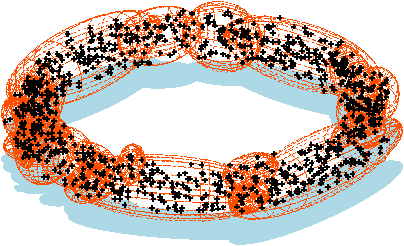
\includegraphics[width=\textwidth]{figures/multinest}
        \texttt{UltraNest}~\arxiv{2101.09604}
        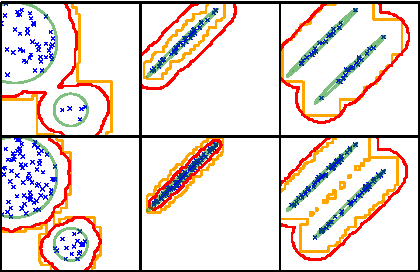
\includegraphics[width=\textwidth]{figures/radfriends}
        \texttt{nautilus}~\arxiv{2306.16923} 
        \texttt{nessai}~\arxiv{2102.11056}
        \texttt{nora}~\arxiv{2305.19267}
        \column{0.43\textwidth}
        \texttt{PolyChord}~\arxiv{1506.00171}
        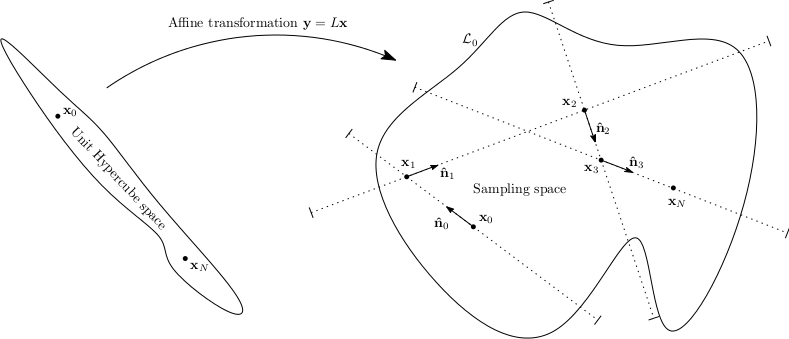
\includegraphics[width=\textwidth]{figures/polychord}
        \vfill
        \texttt{NeuralNest}~\arxiv{1903.10860}
        \begin{columns}
            \column{0.55\textwidth}
            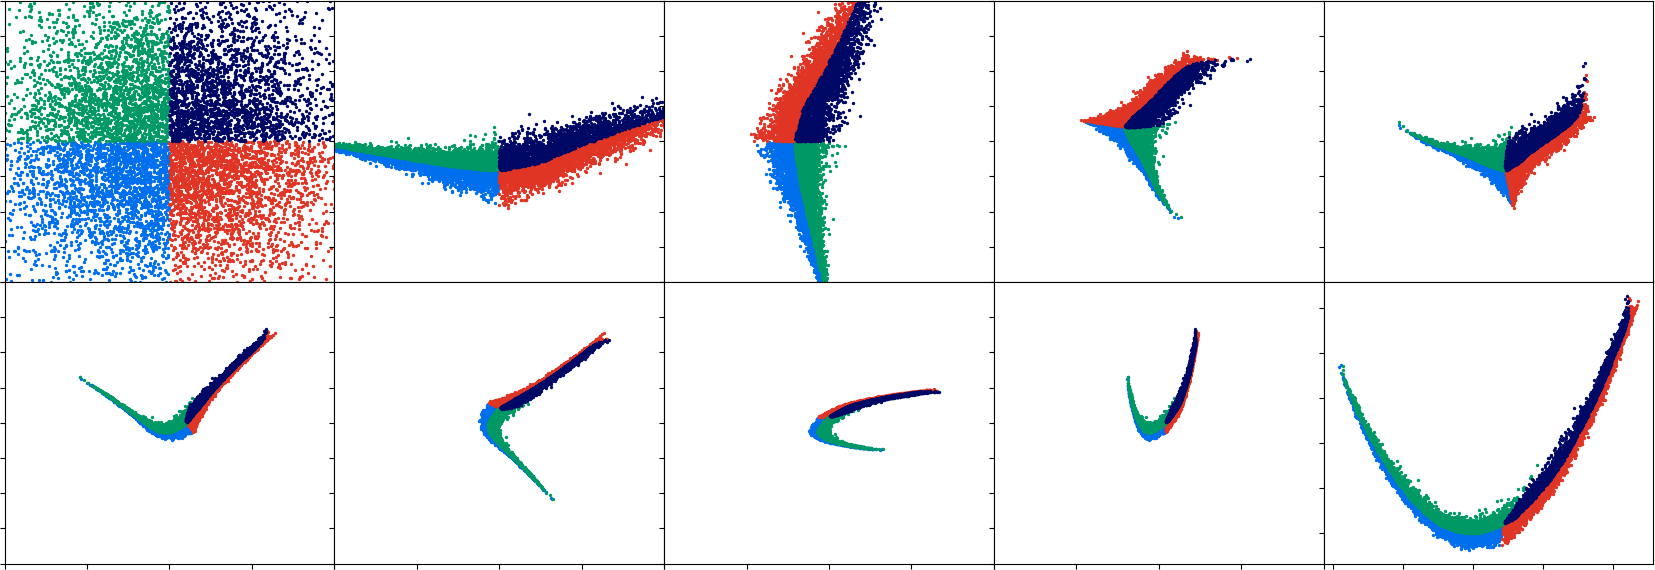
\includegraphics[width=\textwidth]{figures/rosenbrock_flow.png}
            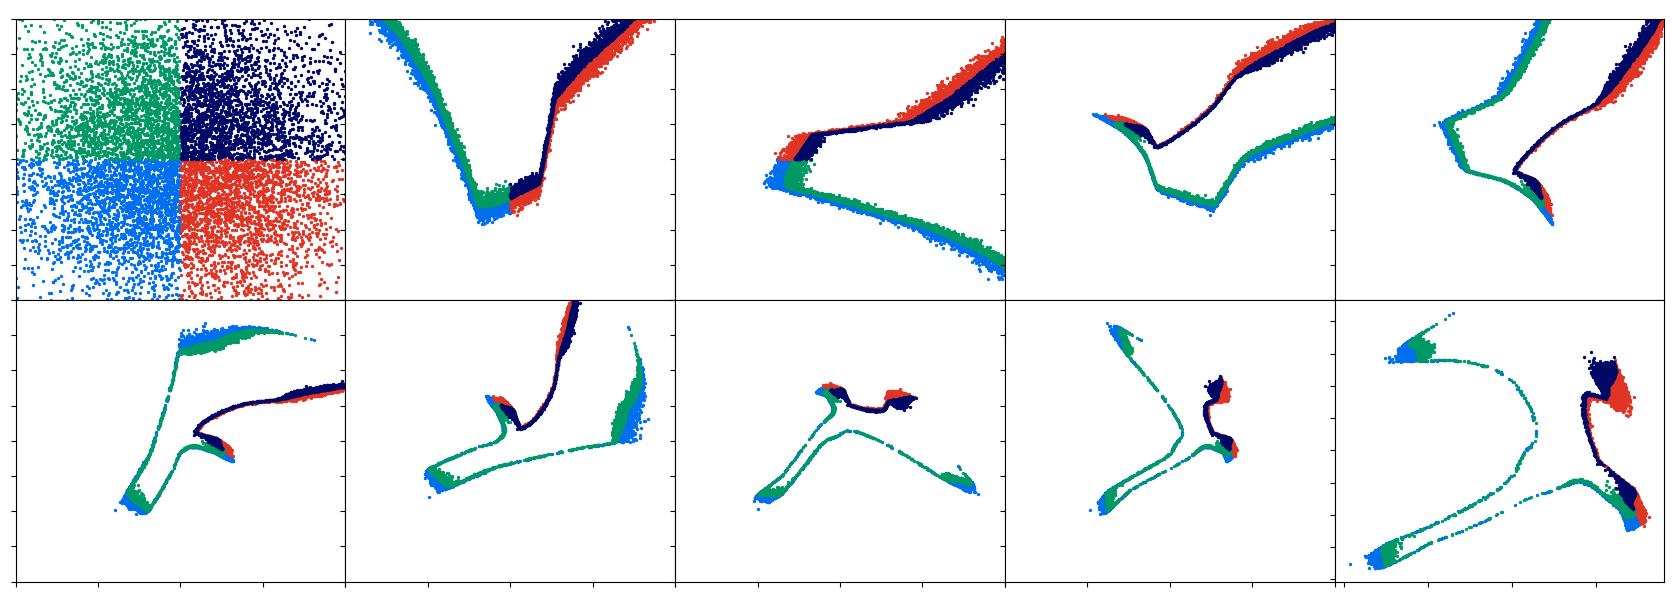
\includegraphics[width=\textwidth]{figures/himmelblau_flow.png}
            \column{0.45\textwidth}
            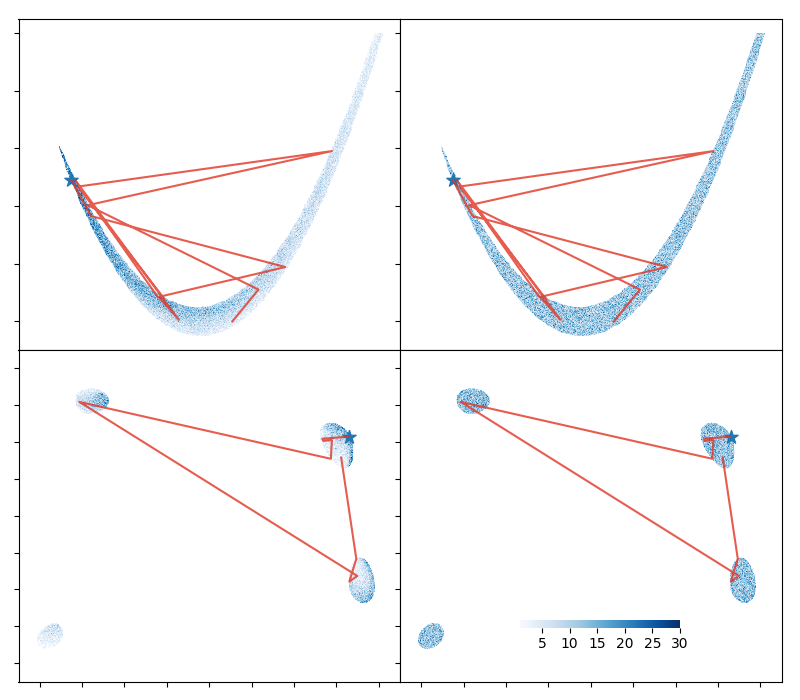
\includegraphics[width=\textwidth]{figures/chains.png}
        \end{columns}
        {\small
            \texttt{jaxns}~\arxiv{2012.15286} \texttt{dynesty}~\arxiv{1904.02180} 
            \texttt{BayesicFitting}~\arxiv{2109.11976}
        }
        \vfill
        \column{0.25\textwidth}
        \texttt{DNest}~\arxiv{1606.03757}
        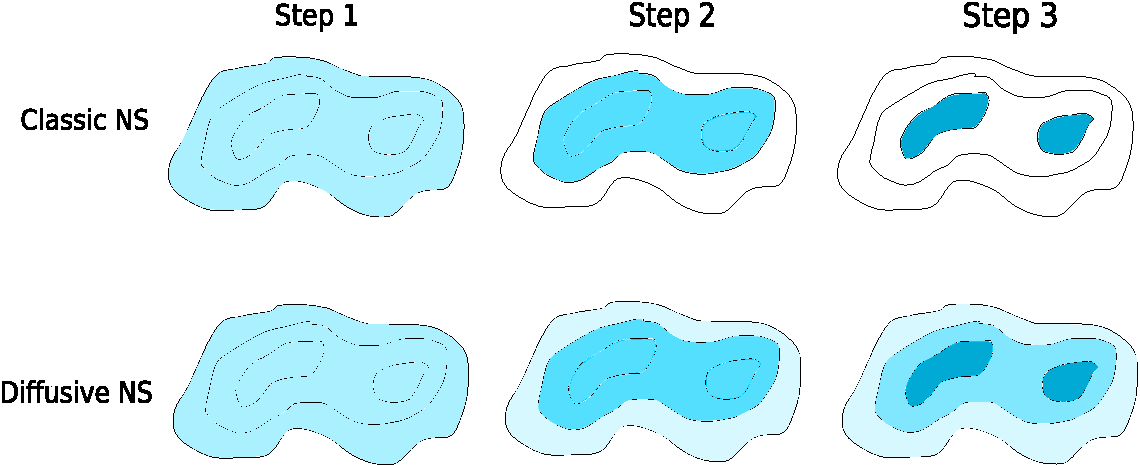
\includegraphics[width=\textwidth]{figures/dnest}
        \texttt{ProxNest}~\arxiv{2106.03646}
        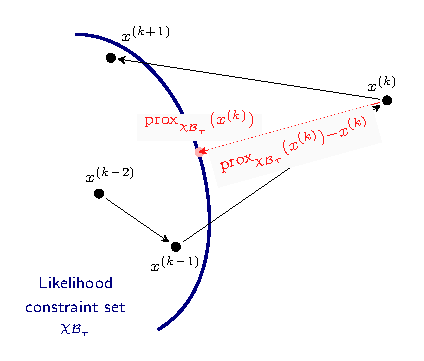
\includegraphics[width=\textwidth]{figures/proxnest_diagram}
        \texttt{nested\_fit}~\arxiv{1611.10189}
        \texttt{pymatnext}~\arxiv{0906.3544}
        \vfill
    \end{columns}
\end{frame}

\begin{frame}
    \frametitle{$f_\text{sampler}$: live-point generation efficiency}
    \begin{itemize}
        \item Broadly, most nested samplers can be split into how they create new live points.
        \item i.e. how they sample from the hard likelihood constraint $\{\theta\sim \C[1]{\pi} : \C[2]{\mathcal{L}}(\theta)>\C[2]{\mathcal{L}_*} \}$.
    \end{itemize}
    \vspace{-10pt}
    \begin{columns}[t]
        \column{0.48\textwidth}
        \begin{block}{Rejection samplers}
            \begin{itemize}
                \item e.g. \texttt{MultiNest}, \texttt{UltraNest}.
                \item Constructs bounding region and draws many invalid points until $\C[2]{\mathcal{L}}(\theta)>\C[2]{\mathcal{L}_*}$.
                \item Efficient in low dimensions, exponentially inefficient $\sim\mathcal{O}(e^{d/d_0})$ in high  $d>d_0\sim10$.
            \end{itemize}
        \end{block}
        \column{0.48\textwidth}
        \begin{block}{Chain-based samplers}
            \begin{itemize}
                \item e.g. \texttt{PolyChord}, \texttt{ProxNest}.
                \item Run Markov chain starting at a live point, generating many valid (correlated) points.
                \item Linear $\sim\mathcal{O}(d)$ penalty in decorrelating new live point from the original seed point.
            \end{itemize}
        \end{block}
    \end{columns}
    \vspace{5pt}
    \begin{itemize}
        \item for high dimensions, state of the art is linear
        \item Recent innovations in \texttt{UltraNest} allow self-tuning of efficiency for rejection sampling
    \end{itemize}
    \begin{alertblock}{Frontier}
        Can chain-based NS self-tune chain length to be sub-linear at run time?
    \end{alertblock}
\end{frame}

\begin{frame}
    \frametitle{$n_\text{live}$: the number of live points}
    \begin{columns}
        \column{0.75\textwidth}
        There are two reasons one might increase the number of live points:
        \begin{block}{Multimodality}
            At each iteration, if a mode has a basin of attraction $<1/n_\text{live}$ of the space you are more likely than not to miss it
            {\small
                \begin{itemize}
                    \item No reason to expect multimodality to have anything so simple as linear scaling with dimension.
                \end{itemize}
            }
        \end{block}
        \vspace{-5pt}
        \begin{block}{Accuracy}
            Evidence error $\sigma(\log \C[3]{\mathcal{Z}}) = \sqrt{\mathcal{D}_\text{KL}/n_\text{live}} $
            {\small
                \begin{itemize}
                    \item So if $\mathcal{D}_\text{KL} \sim \mathcal{O}(d)$, then to maintain the same quality of inference have to scale $n_\text{live}$ at the same rate.
                \end{itemize}
            }
        \end{block}
        \begin{alertblock}{Frontier}
            Can we make this ``mode missing'' argument more quantitative?
        \end{alertblock}
        \column{0.25\textwidth}
        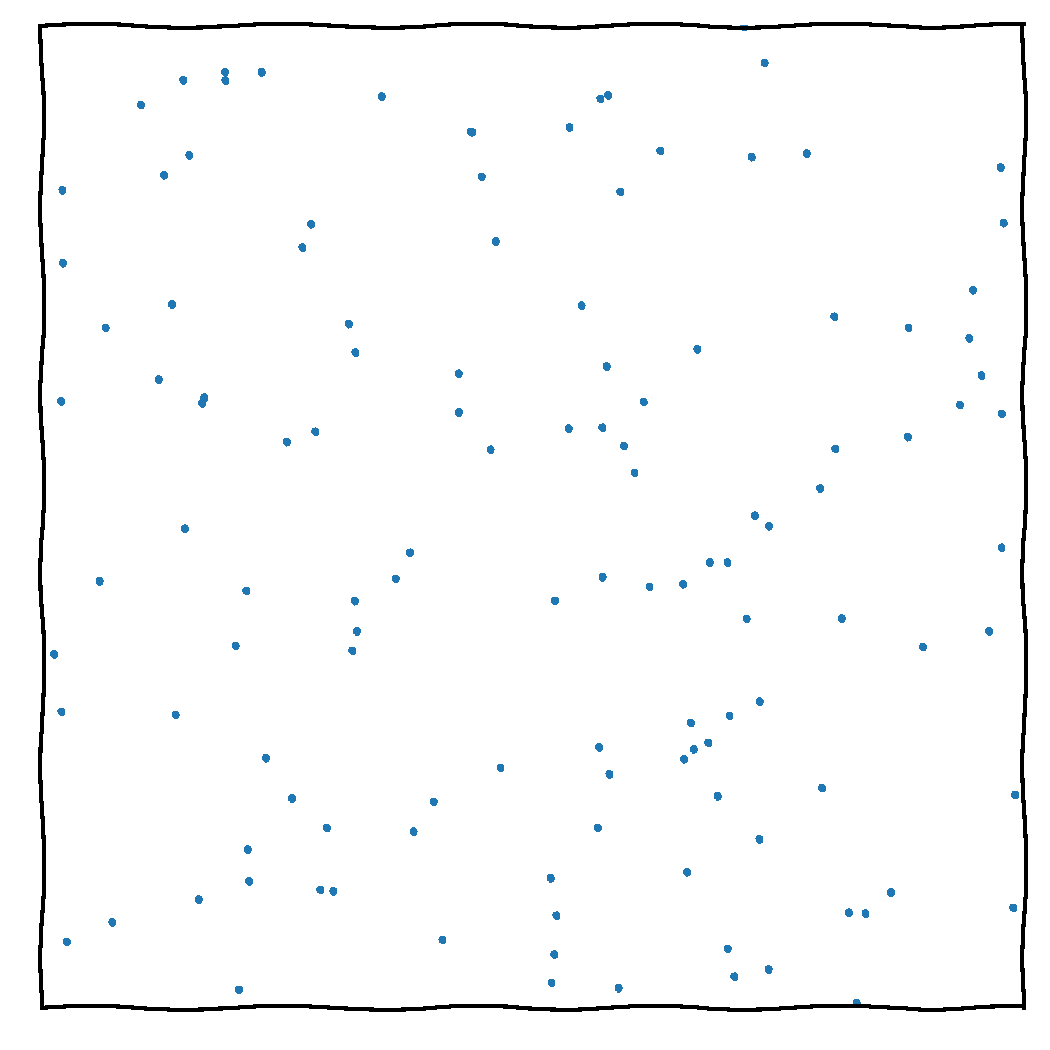
\includegraphics[width=\textwidth,page=1]{figures/himmelblau}
        \includegraphics[width=\textwidth,page=6]{figures/himmelblau}
    \end{columns}
\end{frame}

\begin{frame}
    \frametitle{$T_{\C[2]{\mathcal{L}}}$: the time to evaluate the likelihood}
    \begin{columns}
        \column{0.42\textwidth}
        \begin{block}{Acceleration/emulation}
            \begin{itemize}
                \item Increasing emphasis of using machine learning/AI emulators to accelerate slow components of pipelines
                \item Nested sampling dead points are good at training emulators of likelihoods, due to their nose-to-tail sampling (Brewer's ``Dead measure'')
                \item \texttt{BAMBI}~\arxiv{1110.2997} does this at run-time to accelerate nested sampling
            \end{itemize}
        \end{block}
        \begin{alertblock}{Frontier}
            Is BAMBI the best we can do?
        \end{alertblock}
        \column{0.135\textwidth}
        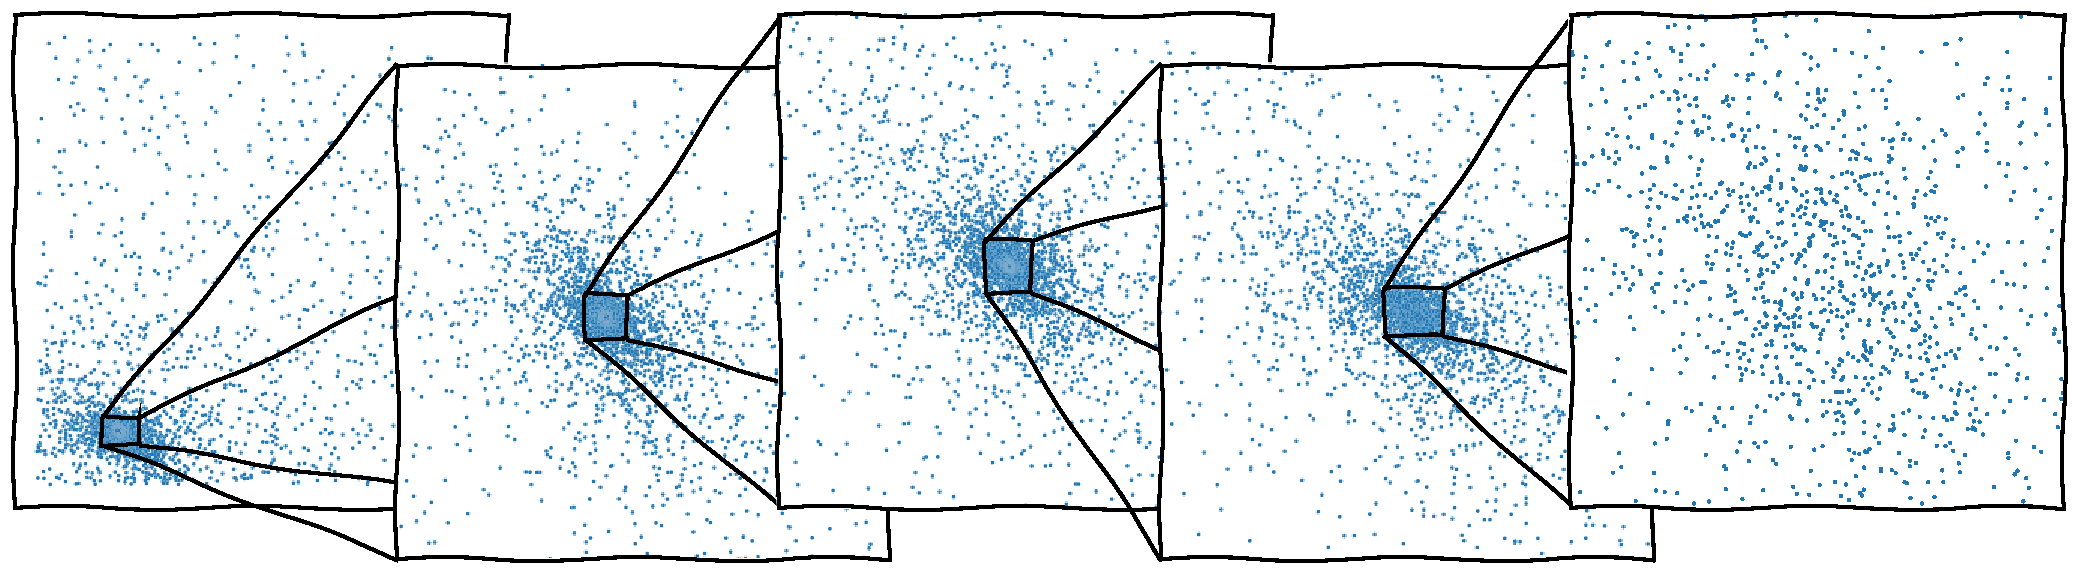
\includegraphics[angle=-90,width=\textwidth]{figures/dead_measure}
        \column{0.42\textwidth}
        \begin{block}{Fast-slow hierarchies}
            \begin{itemize}
                \item Success in cosmology where some parameters take longer than others
                \item reduces $T_{\C[2]{\mathcal{L}}}\sim\mathcal{O}(d_\text{slow})$.
            \end{itemize}
        \end{block}
        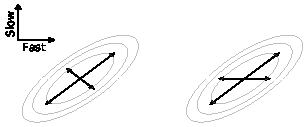
\includegraphics[width=\textwidth]{figures/fast_slow.pdf}
        \begin{alertblock}{Frontier}
            Can fast-slow hierarchies be better automated within algorithms?
        \end{alertblock}
    \end{columns}
\end{frame}

\begin{frame}
    \frametitle{$\mathcal{D}_\text{KL}$: The Kullback Leibler divergence}
    \begin{columns}
        \column{0.75\textwidth}
        \begin{itemize}
            \item Naively $\mathcal{D}_\text{KL} \sim \mathcal{O}(d)$, since if you have $d$ \emph{useful} parameters, you would expect to need to compress each of them, so each contribute linearly to the volume contribution
            \item From the Occam's razor equation however:
                \[\log \C[3]{\mathcal{Z}} = \av[{\mathcal{P}}]{\log\C[2]{\mathcal{L}}} - \mathcal{D}_\text{KL}\]
                a large $\mathcal{D}_\text{KL}$ means a ``bad'' model
            \item Methods which explore models weighted by their evidence won't spend as much time in high $\mathcal{D}_\text{KL}$ regions~\arxiv{1506.09024}.
            \item There's also an intuition of the KL being ``information'', so increasing the number of parameters shouldn't extract more content.
            \item The KL divergence is a property of the model, so one would initially consider this to be something that the user has no control over\ldots
        \end{itemize}
        \column{0.25\textwidth}
        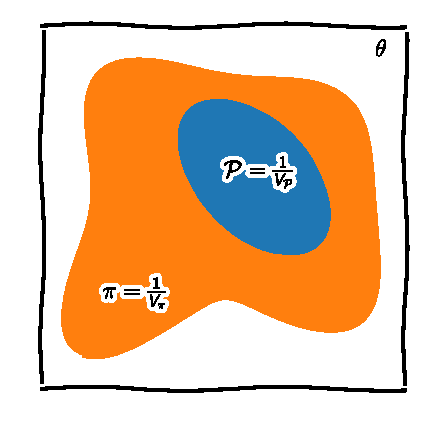
\includegraphics[width=\textwidth]{figures/volumes.pdf}
        \[ \mathcal{D}_\text{KL} = \log \frac{V_{\C[1]{\pi}}}{V_{\C[0]{\mathcal{P}}}} \]
        \[ \mathcal{D}_\text{KL} = \av[{\C[0]{\mathcal{P}}}]{\log\frac{\C[0]{\mathcal{P}}}{\C[1]{\pi}}} \]
    \end{columns}
\end{frame}

\begin{frame}
    \frametitle{Posterior repartitioning}
    \student{aleksandr_petrosyan}{Aleksandr Petrosyan}{MSci 2021}
    \begin{columns}
        \column{0.5\textwidth}
        \begin{itemize}
            \item Almost all sampling algorithms (MH, HMC, SMC) are only sensitive to the product of likelihood and prior $\boxed{\C[2]{\mathcal{L}}\times\C[1]{\pi}}$.
            \item In practice this manifests as many codes implementing ``prior terms'' in the likelihood (or visa-versa) with no ill effect
        \item Nested sampling is unusual, in that one ``samples from the prior $\C[1]{\pi}$, subject to a hard constraint $\C[2]{\mathcal{L}}>\C[2]{\mathcal{L}_*}$.'':
                \[\{\theta\sim \C[1]{\pi} : \C[2]{\mathcal{L}}(\theta)>\C[2]{\mathcal{L}_*} \}\] 
            \item This separates the prior from the likelihood at an algorithmic level.
        \end{itemize}
        \column{0.5\textwidth}
        \begin{itemize}
\item One can therefore repartition the likelihood and prior $(\C[2]{\mathcal{L}},\C[1]{\pi})\to(\C[2]{\tilde{\mathcal{L}}},\C[1]{\tilde{\pi}})$, providing
                \[ \boxed{\C[2]{\mathcal{L}}\times\C[1]{\pi} = \C[2]{\tilde{\mathcal{L}}}\times\C[1]{\tilde{\pi}}}\]
            \item This moves pieces between likelihood and prior that you have analytic control over.
                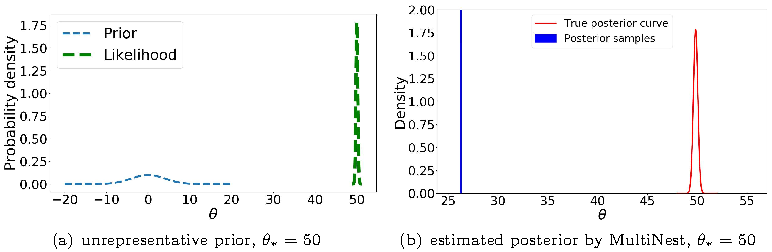
\includegraphics[width=\textwidth]{figures/repartition}
            \item Chen, Feroz \& Hobson~\arxiv{1908.04655} invented this to deal with misspecified priors
        \end{itemize}
    \end{columns}
\end{frame}

\begin{frame}
    \frametitle{Posterior repartitioning for acceleration}
    \student{metha_prathaban}{Metha Prathaban}{PhD}
    \begin{columns}
        \column{0.5\textwidth}
        \begin{exampleblock}{Key idea}
Whilst posteriors and evidences are invariant to repartitioning $\C[2]{\mathcal{L}}\to\C[2]{\tilde{\mathcal{L}}}$, the KL divergence is not.
        \end{exampleblock}
    \begin{itemize}
            \item For constant ``run quality'' $\sigma$, 
            \begin{gather*} 
                {\scriptstyle
                    T = T_{\C[2]{\mathcal{L}}} \times n_\text{live} \times \mathcal{D}_\text{KL} \times f_\text{sampler}, \quad
\sigma \approx \sqrt{\mathcal{D}_\text{KL}/n_\text{live}} }
    \\
\Rightarrow\boxed{T = T_{\C[2]{\mathcal{L}}} \times \sigma \times \mathcal{D}_\text{KL}^2 \times f_\text{sampler}} 
        \end{gather*}
            so if you can reduce the KL divergence, then quadratic gains to be made
        \item \texttt{SuperNest}~\arxiv{2212.01760}
        \item Ongoing work with Metha Prathaban \& Harry Bevins.
    \end{itemize}
        \column{0.5\textwidth}
        \vspace{8pt}
        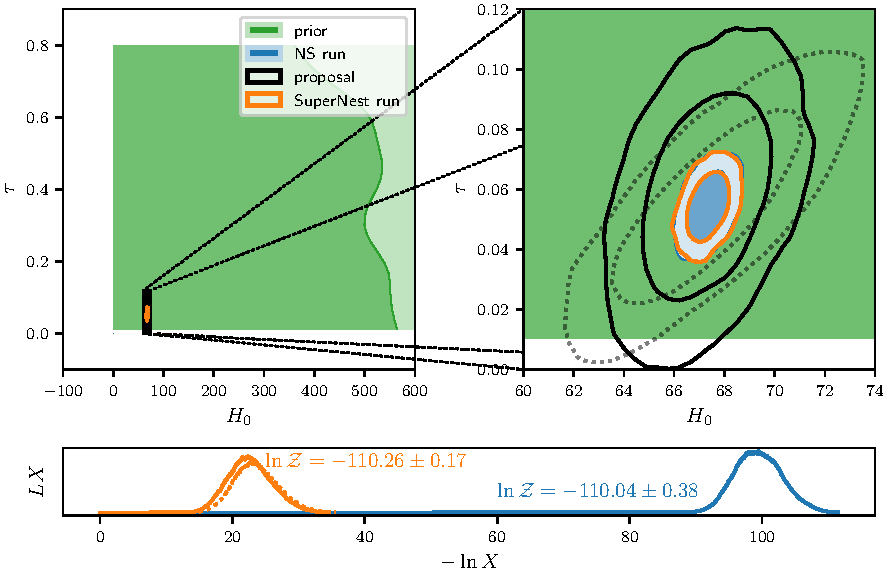
\includegraphics[width=\textwidth]{figures/supernest.pdf}
    \begin{alertblock}{Frontier}
        Can we use posterior repartitioning to quadratically reduce the run time of nested sampling?
    \end{alertblock}
    \end{columns}
\end{frame}

\begin{frame}
    \frametitle{Parallelisation}
    \begin{columns}
        \column{0.5\textwidth}
        \begin{itemize}
            \item Nested sampling is well-suited to parallelisation, up to the number of live points, in contrast with MH/HMC
            \item I've known people run nested sampling on 10,000 CPUs
            \item This is in addition to any existing parallelisation in the likelihood
            \item Dynamic nested sampling very useful here adding machinery for throwing away multiple points~\arxiv{1704.03459}
        \end{itemize}
        \begin{alertblock}{Frontier}
            Are there any other parallelisation strategies, e.g. clustering/divide \& conquer?
        \end{alertblock}
        \column{0.5\textwidth}
        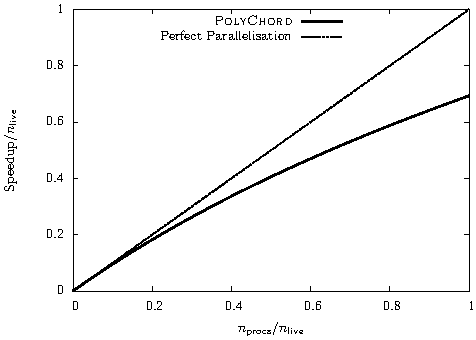
\includegraphics[width=\textwidth]{figures/parallelisation}
    \end{columns}
\end{frame}

\begin{frame}
    \frametitle{Nested sampling with gradients}
    \student{namu_kroupa}{Namu Kroupa}{PhD (with Gábor Csányi)}
    \begin{columns}
        \column{0.5\textwidth}
        \begin{itemize}
            \item  In principle, gradients give you $\sim\mathcal{O}(d)$ pieces of information to help with exploration
            \item With modern automatic differentiation codes (\texttt{JAX}, \texttt{PyTorch}, \texttt{TensorFlow}, \texttt{Enzyme} \ldots)
                    \\ these now come ``for free''.
            \item However nested sampling has unique challenges, so plugging in default (e.g. HMC/Langevin) algorithms does not work
        \end{itemize}
        \begin{alertblock}{Frontier}
            Can you come up with a nested sampling strategy that uses gradients and scales pass $d\sim\mathcal{O}(100)$?
        \end{alertblock}
        \column{0.5\textwidth}
        \vspace{6pt}
        \includegraphics<1|handout:3>[width=\textwidth,page=1]{figures/himmelblau_gradient}%
        \includegraphics<2|handout:3>[width=\textwidth,page=2]{figures/himmelblau_gradient}%
        \includegraphics<3|handout:3>[width=\textwidth,page=3]{figures/himmelblau_gradient}%
        \includegraphics<4|handout:3>[width=\textwidth,page=4]{figures/himmelblau_gradient}%
        \includegraphics<5|handout:3>[width=\textwidth,page=5]{figures/himmelblau_gradient}%
        \includegraphics<6|handout:3>[width=\textwidth,page=6]{figures/himmelblau_gradient}%
    \end{columns}
\end{frame}

\begin{frame}
    \frametitle{Nested sampling with gradients}
    \student{namu_kroupa}{Namu Kroupa}{PhD (with Gábor Csányi)}
    \begin{description}
        \item[Betancourt] Hamiltonian constrained nested sampling~\arxiv{1005.0157}.
        \item[Feroz] Galilean Nested Sampling~\arxiv{1312.5638}.
        \item[Skilling] Galilean and Hamiltonian Monte Carlo~\doi{10.3390/proceedings2019033019}
        \item[Speagle] Incorporated into \texttt{dynesty}~\arxiv{1904.02180}.
        \item[Habeck] Habeck Demonic nested sampling -- uses thermodynamic analogy to soften the hard boundary with a Maxwell daemon~\doi{10.1063/1.4905971}.
        \item[Baldock] Total Enthalpy HMC, incorporating momenta in a more HMC like way, but specialised to materials science~\arxiv{1710.11085}.
        \item[Cai] ProxNest for high-dimensional convex imaging problems~\arxiv{2106.03646}.
        \item[Lemos] Updated existing HMC/Galilean nested sampling to use differentiable programming (jax/torch) ICML 2024~\arxiv{2312.03911}
    \end{description}
    \begin{itemize}
        \item See also 2023 MIAPbP talk ``Gradients and nested sampling: The present state of the art''
        \item Come talk to me afterwards for further detail on what I'm working on with Namu Kroupa.
    \end{itemize}
\end{frame}

\begin{frame}
    \frametitle{Reversible nested sampling}
    \begin{columns}
        \column{0.5\textwidth}
\vspace{-10pt}
        \begin{itemize}
            \item One could in principle reverse the direction of travel, and move outward from a peak.
            \item Need to know the initial volume $X_\text{start}\ne1$
            \item e.g. if a Laplace estimation were good enough at the peak.
            \item The same trick in normal nested sampling would reduce volume estimation error and hence improve scaling.
        \end{itemize}
        \begin{alertblock}{Frontier}
            \begin{itemize}
                \item Can you come up with a reversible nested sampling algorithm?
                \item Can you reduce the volume estimation error by clamping the end point?
            \end{itemize}
        \end{alertblock}
        
        \column{0.5\textwidth}
        \includegraphics<1>[width=\textwidth,page=7]{figures/himmelblau}%
        \includegraphics<2|handout:0>[width=\textwidth,page=6]{figures/himmelblau}%
        \includegraphics<3|handout:0>[width=\textwidth,page=5]{figures/himmelblau}%
        \includegraphics<4|handout:0>[width=\textwidth,page=4]{figures/himmelblau}%
        \includegraphics<5|handout:0>[width=\textwidth,page=3]{figures/himmelblau}%
        \includegraphics<6|handout:0>[width=\textwidth,page=2]{figures/himmelblau}%
        \includegraphics<7-|handout:0>[width=\textwidth,page=1]{figures/himmelblau}%
    \end{columns}
\end{frame}

\begin{frame}
    \frametitle{Memory scaling}
    \student{adam_ormondroyd}{Adam Ormondroyd}{PhD}
    \begin{columns}
        \column{0.4\textwidth}
    \begin{itemize}
        \item Memory is driven by needing to store:
            \begin{itemize}
                \item dead points $n_\text{dead}=n_\text{live}\times\mathcal{D}_\text{KL}\sim \mathcal{O}(d^2)$
                \item optionally their coordinates $\sim\mathcal{O}(d)$
                \item optionally further machinery for generating new live points $\sim\mathcal{O}(d)$
            \end{itemize}      
        \item \texttt{anesthetic}~\arxiv{1905.04768} as a performant tool for post-processing nested sampling runs
    \end{itemize}
        
        \column{0.6\textwidth}
        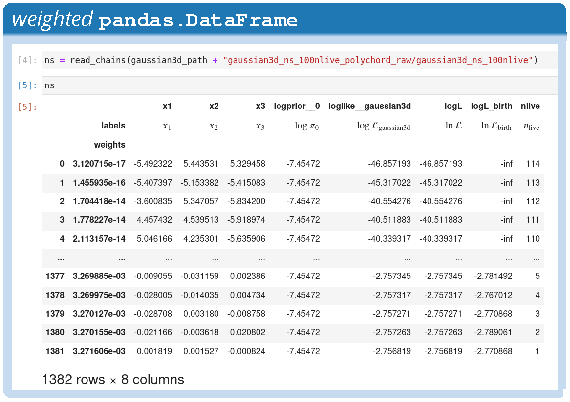
\includegraphics[width=\textwidth]{figures/dataframe}
    \end{columns}
\end{frame}

\begin{frame}
    \frametitle{Conclusions}
    \framesubtitle{\tthref{github.com/handley-lab}}

    \begin{columns}[t]
        \column{0.47\textwidth}
        \begin{block}{How fast in nested sampling?}
            \[ \boxed{T = T_{\C[2]{\mathcal{L}}} \times n_\text{live} \times \mathcal{D}_\text{KL} \times f_\text{sampler}} \]
        \end{block}
        \column{0.43\textwidth}
        \begin{block}{How accurate is nested sampling?}
            \[ \boxed{\sigma(\log\C[3]{\mathcal{Z}}) \approx \sqrt{\mathcal{D}_\text{KL}/n_\text{live}}} \]
        \end{block}
    \end{columns}

    \begin{columns}
        \column{0.5\textwidth}
        \begin{itemize}
            \item Scaling on the face of it $T\sim\mathcal{O}(d^4)$
            \item In reality can be anywhere between $T\sim\mathcal{O}(d_\text{slow})$ and $T\sim\mathcal{O}(d^4)$
            \item Memory scaling $\sim\mathcal{O}(d^{2-4})$
            \item Most people focus on improving $f_\text{sampler}$, but this is only a fraction of the story.
            \item Large accelerations to be made in the other terms
        \end{itemize}
        \column{0.5\textwidth}
        \begin{itemize}
            \item Technical Review paper: Buchner \arxiv{2101.09675}
            \item Nature Review paper: \arxiv{2205.15570}
            \item \texttt{aeons}~\arxiv{2312.00294}
            \item \texttt{SuperNest}~\arxiv{2212.01760}
        \end{itemize}
    \end{columns}


    \tikz[overlay,remember picture]
    \node[anchor=north east] (A) at ($(current page.north east)+(0,0)$) {
        
\includegraphics[width=0.09\textheight]{figures/students/adam_ormondroyd.jpg}%
        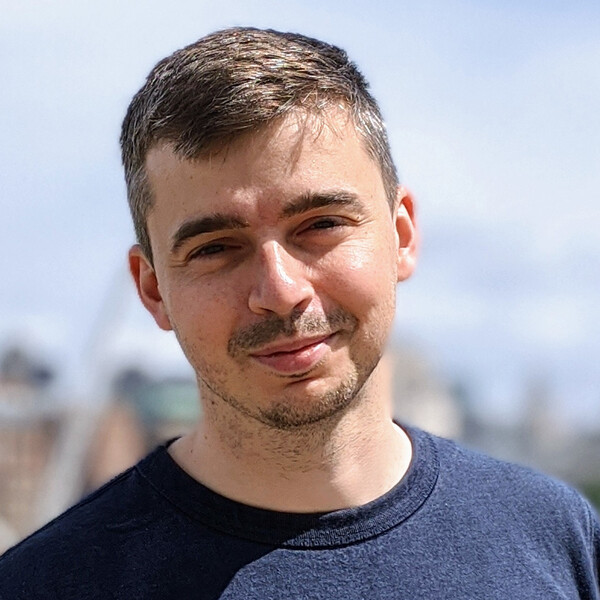
\includegraphics[width=0.09\textheight]{figures/students/david_yallup.jpg}%
        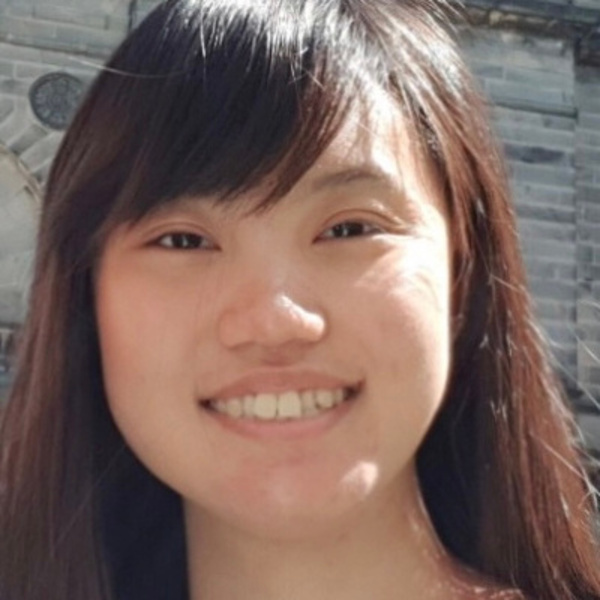
\includegraphics[width=0.09\textheight]{figures/students/dily_ong.jpg}%
        
\includegraphics[width=0.09\textheight]{figures/students/george_carter.jpg}%
        
\includegraphics[width=0.09\textheight]{figures/students/harry_bevins.jpg}%
        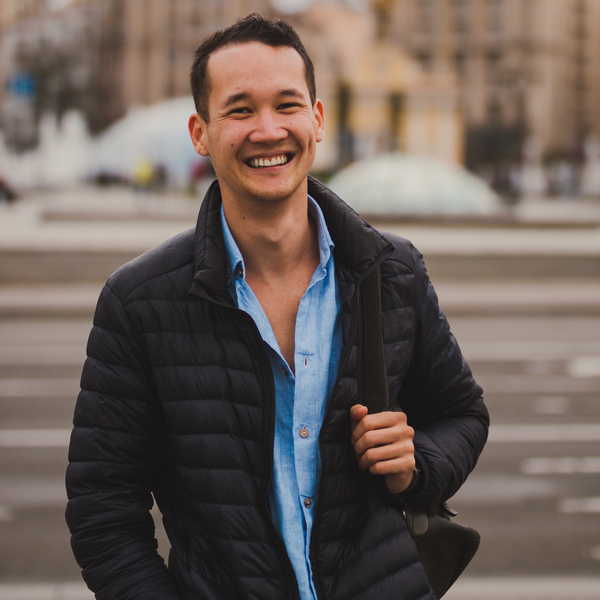
\includegraphics[width=0.09\textheight]{figures/students/kilian_scheutwinkel.jpg}%
        
\includegraphics[width=0.09\textheight]{figures/students/metha_prathaban.jpg}%
        
\includegraphics[width=0.09\textheight]{figures/students/namu_kroupa.jpg}%
        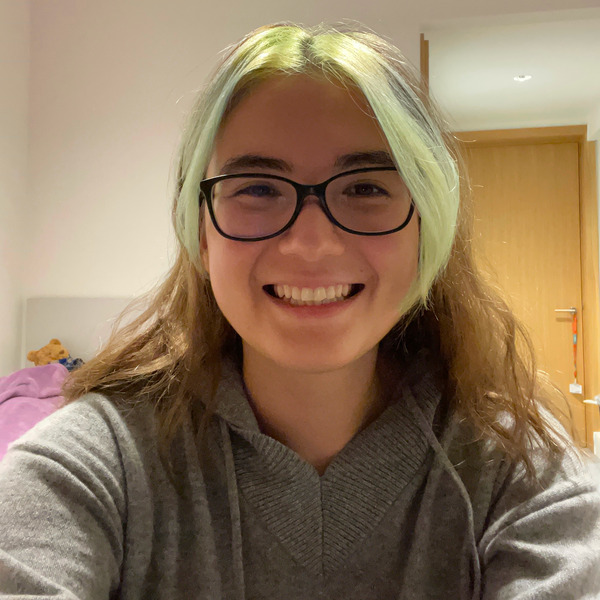
\includegraphics[width=0.09\textheight]{figures/students/sinah_legner.jpg}%
        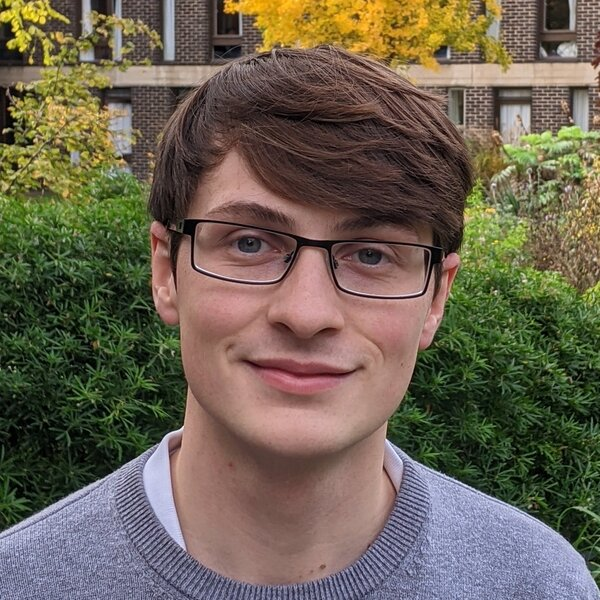
\includegraphics[width=0.09\textheight]{figures/students/thomas_gessey-jones.jpg}%
        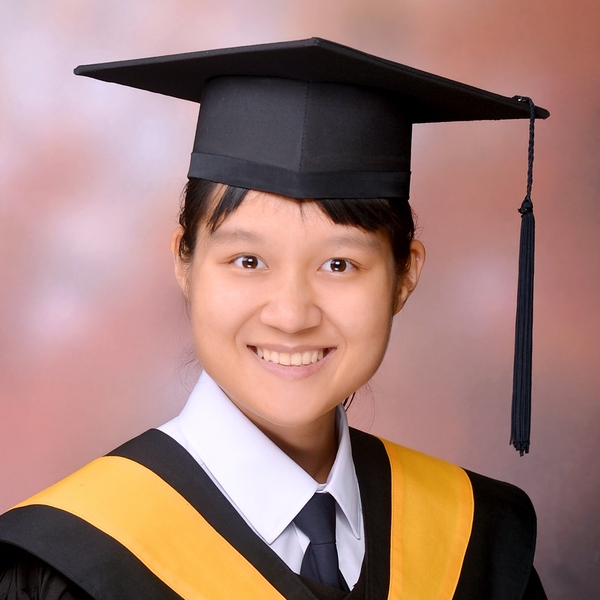
\includegraphics[width=0.09\textheight]{figures/students/wei-ning_deng.jpg}%
    };
\end{frame}

\appendix
\begin{frame}
    \frametitle{Probabalistic volume estimation}
    \begin{columns}
        \column{0.5\textwidth}
        \begin{itemize}
            \item Key idea in NS: estimating volumes probabilistically
                \[
                    \only<-2>{
                        \frac{\C[1]{V_\text{after}}}{\C[0]{V_\text{before}}} 
                        \approx \frac{\C[1]{n_\text{in}}}{\C[0]{n_\text{out}}+\C[1]{n_\text{in}}}
                    }
                    \only<3>{
                        \frac{\C[1]{V_\text{after}}}{\C[0]{V_\text{before}}} 
                        \approx \frac{\C[1]{n_\text{in}}+1}{\C[0]{n_\text{out}}+\C[1]{n_\text{in}}+2}
                    }
                    \only<4>{\hspace{-15pt}
                        \frac{\C[1]{V_\text{after}}}{\C[0]{V_\text{before}}} 
                        \sim \frac{\C[1]{n_\text{in}}+1}{\C[0]{n_\text{out}}+\C[1]{n_\text{in}}+2} \pm \sqrt{\tfrac{(\C[1]{n_\text{in}}+1)(\C[0]{n_\text{out}}+1)}{(\C[0]{n_\text{out}}+\C[1]{n_\text{in}}+2)^2(\C[0]{n_\text{out}}+\C[1]{n_\text{in}}+3)}}
                    }
                \]
            \item This is the \textbf{only} way to calculate volume in high dimensions $d>3$.
                \begin{itemize}
                    \item Geometry is exponentially inefficient.
                \end{itemize}
            \item This estimation process does not depend on geometry, topology or dimensionality
            \item Basis of all Monte-Carlo integration
            \item Nested Sampling uniquely uses a nested framework to couple together MC integrals in a robust, scalable manner.
        \end{itemize}
        \column{0.5\textwidth}
        \includegraphics<1>[width=\textwidth]{figures/compression_1}%
        \includegraphics<2->[width=\textwidth]{figures/compression_2}%
    \end{columns}
\end{frame}

\begin{frame}
    \frametitle{Why dynamic nested sampling doesn't help}
    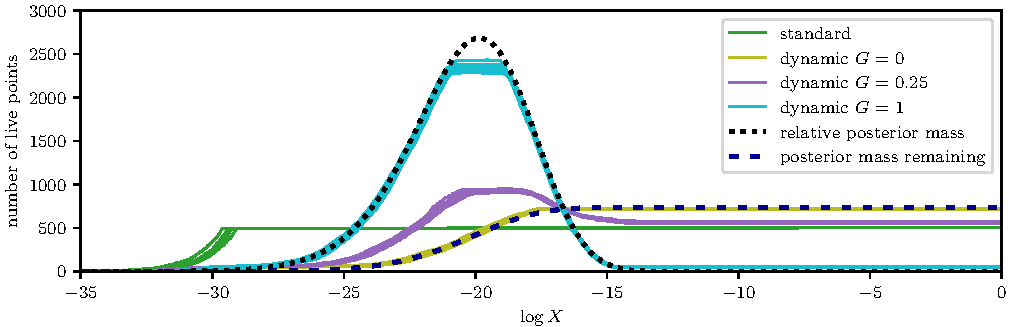
\includegraphics[width=\textwidth]{figures/dynamic}
    \vspace{-20pt}
    \begin{columns}
        \column{0.5\textwidth}
        \begin{itemize}
            \item In dynamic nested sampling~\arxiv{1704.03459}, live points are varied by choosing to optionally create/delete at each iteration.
            \item Can use this to ``focus'' computational power on posterior.
        \end{itemize}
        \column{0.5\textwidth}
        \begin{itemize}
            \item However, this is at the cost of reducing evidence accuracy.
            \item Equivalent to saying ``We could just set $n_\text{live}$ very low'' as a solution to scaling.
        \end{itemize}
    \end{columns}
\end{frame}

\end{document}
